
\chapter{Lecture 4}

\subsection{Common fallacies}

\begin{itemize}
	\item
		Confusion of inverses, i.e.~$P(A\mid B) \simeq P(B\mid A)$, in general is \emph{not} true.
		Since $P(A\mid B)\,P(B) = P(B\mid A)\,P(A)$, the previous relation is \emph{only} true if $P(A)\simeq P(B)$.
	\item
		Assuming that $P(A)\simeq P(A\mid B)$.
		From the law of total probability $P(A) = P(A\mid B)\,P(B) + P(A\mid \bar B)\,P(\bar B)$.
		For instance, if a doctor estimates the probability for a person of having a flue $P(\text{flue})$ by counting how many of his patients have it, he actually estimates $P(\text{flue}\mid\text{sees doctor})$: this is an example of selection bias.
	\item
		Base rate neglect: not taking into account the prior $P(A)$.
\end{itemize}


\section{Bayesian interpretation: subjective probability}

Unlike the frequentist interpretation of probability, the Bayesian one provides a more natural treatment of non-repeatable phenomena.

The probability is the state of knowledge assigned to the hypothesis, i.e.~the statement that they are true or false.
So let's call $P(A)$ the degree of belief that $A$ is true.
Bayes' theorem is a \emph{learning rule}: it expresses how the subjective degree of belief has to be updated in view of new data (or \emph{evidence}).


Typically, one says $A = \text{theory}$ and $B = \text{data}$ so that~\eqref{eq:bayes_theorem} reads
\begin{equation}
	P(\text{theory}\mid\text{data}) = \frac{P(\text{data}\mid \text{theory})\,P(\text{theory})}{P(\text{data})}.
\end{equation}
The probability for the theory of being true \emph{after} seeing the data $P(\text{theory}\mid\text{data})$ is called \emph{posterior probability}\index{probability!posterior}\index{posterior}.
The probability that the theory is true \emph{before} seeing the data $P(\text{theory})$ is called \emph{prior probability}\index{probability!prior}\index{prior}.
The probability of observing certain data given that the theory is true $P(\text{data}\mid \text{theory})$ is called \emph{likelihood of hypothesis}\index{likelihood!of hypothesis}.
The probability of observing the data assuming that \emph{every} theory is true $P(\text{data})$ is called \emph{evidence}\index{evidence}.


If the theory predicts data with high probability (i.e.~hypothesis likelihood is high) and the data are not likely (i.e.~evidence is small) than the observation will straighten the belief in the theory.
On the other hand, the observation of data which are forbidden by the theory will disprove the theory itself since $P(\text{data}\mid \text{theory}) = 0$ and so will be $P(\text{theory}\mid\text{data})$.


Using now a continuous form of the law of total probability we can introduce an integration over all possible hypothesis
\begin{equation}
	P(t\mid d) = \frac{P(d\mid t)\,P(t)}{\int P(d\mid t')\,P(t')\ud t'}.
\end{equation}
So we have a clear separation between the prior belief and the outcome of the measurement.
Moreover the posterior probability is proportional to the prior probability.


Bayes' theorem is a powerful tool but it does not say how to assign probabilities, i.e.~how to choose priors, hence it reflect a subjective belief.
It is just an ``if-then'' statement:
\begin{description}
	\item[if]
		I choose $P(\text{theory})$ and perform an experiment which gives a certain set of data;
	\item[then]
		I can update my degree of belief in the theory in the light of the new collected data.
\end{description}


When I collect more data, I can sequentially apply the Bayes' theorem.
The previous posterior $P(t\mid d_1)$ becomes the new prior $P(t)$ for the next knowledge update with $d_2$.


\section{Frequentist vs.~Bayesian}

{\setlength{\epigraphwidth}{%
		\widthof{\epigraphsize%
			Bayesians address the questions everyone is interested%
		}%
	}
	\epigraph{%
		Bayesians address the questions everyone is interested in by using assumptions that no one believes.
		Frequentist use impeccable logic  to deal with an issue that is of no interest to anyone.
	}{\footnotesize%
		%\textsl{Another Brick in the Wall, pt.~2}\\%
		\textsc{louis lyons}%
	}
}

%\epigraph{}{%
%\textsc{}%
%}

\begin{description}
	\item[Frequentist]
		\begin{itemize}
			\item
				The hypothesis are states of nature: they can be either true or false;
			\item
				The prior belief is often hidden: it does not appear explicitly.
		\end{itemize}
	\item[Bayesian]
		\begin{itemize}
			\item
				Probabilities are state of knowledge which are assigned to hypothesis;
			\item
				Prior beliefs enter explicitly but there is usually no consensus on priors;
			\item
				Different priors result in different posteriors;
			\item
				It is a more natural treatment of non-repeatable phenomena e.g.~systematic uncertainties, hypothesis testing and so forth;
			\item
				The posterior probability converges to about the same value after several experiments, irrespective of choice of priors.
		\end{itemize}
\end{description}

\section{\aclp{rv}}

\acp{rv} are variables whose values vary due to some source of randomness---be it our ``ignorance'' on the system or a randomness which lies in the laws of Physics.
They are a numerical characteristics assigned to each element of the sample space (i.e.~functions on $S$) and represent the outcomes of the experiment.
They are a set of possible different values, each associated with a probability.

There are two kinds of \acp{rv}:
\begin{description}
	\item[Discrete] e.g.~the outcomes of throwing a dice;
	\item[Continuous] e.g.~the energy of a particle. In this case, a single value has \emph{null} probability and non-zero probabilities are given only for \emph{ranges} of values.
\end{description}

\section{Probability distributions}

They assign a probability to each possible value of a \ac{rv}, namely to each possible outcome of an experiment.





To a continuous \ac{rv} $X$ with value $x$ is associated a \ac{pdf} $f(x)$ such that
\begin{equation}
	P(X\in[x,x+\ud x]) = f(x)\ud x.
\end{equation}
From here we see that $P(X=x) = 0$ since $\ud x = 0$.
This means that probabilities are non vanishing only for events which involve a range of outcomes, namely probability that the outcome of the experiment is \emph{exactly} $\pi$ is zero but probability that it lies in the range $[\pi,\pi+\epsilon]$ for each (positive) value of $\epsilon = \num{4345}, \num{e-39}$ and so on is not.


Moreover, the probability $P$ is ``just a number'': it's dimensionless.
Thus it's clear that $f(x)$ is a \emph{density} and it has the dimension $1/x$ so it is \emph{not} a probability.


From axioms of probability it follows that $P(x\in\R)$, the sure event, must be equal to \num{1}.
Now, since the probability for the \ac{rv} to lie in finite intervals is obtained just by integrating over the interval, namely
\begin{equation}
	P( X \in [a,b] ) = \int_a^b f(x)\ud x,
\end{equation}
the normalization condition reads
\begin{equation}
	\int_\R f(x)\ud x = 1.
\end{equation}


For a discrete \ac{rv} things are a little different.
First of all, discrete doesn't mean \emph{finite}, e.g.~the harmonic oscillator energies are a discrete and infinite set $\Set{\hbar\omega(n+1/2)}$.
Probability for the outcomes of a discrete \ac{rv} $X$ with values $x$ are described by a \emph{probability mass function}\index{probability!mass function} $\phi(x)$ such that
\begin{equation}
	P(X=x_i) = \phi(x_i),
\end{equation}
namely $\phi$ \emph{is} a probability so it must be non negative.
\begin{figure}
	\centering
	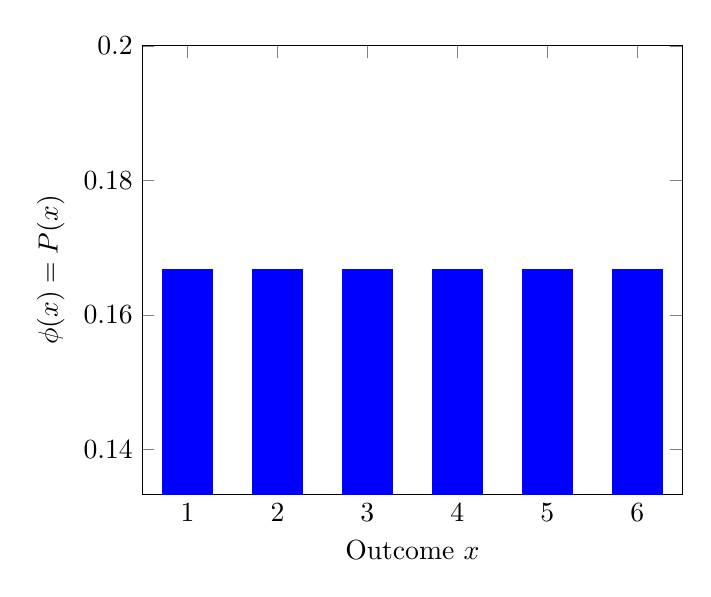
\begin{tikzpicture}
\begin{axis}[
%	ybar interval,
	xlabel = {Outcome $x$},
	ylabel = {$\phi(x) = P(x)$},
  ]
%[
%	xtick={1./6.},
%  	ytick={\pgfmathparse{1./6.}}, %doesn't work
%]
\addplot+[
	ybar,
	fill,
	mark = none,
	bar width=18pt
] coordinates {
(1,1/6)%
(2,1/6)%
(3,1/6)%
(4,1/6)%
(5,1/6)%
(6,1/6)%
};
\end{axis}
\end{tikzpicture}

	\caption{Probability mass function for a rolling dice: every outcome in $\Set{1,\dots,6}$ as $1/6$ probability.}
	\label{fig:dicePMD}
\end{figure}
Figure~\ref{fig:dicePMD} a flat probability distribution for a rolling dice is shown.
The normalization condition reads in this case
\begin{equation}
	1 = \sum_i \phi(x_i).
\end{equation}


A probability mass distribution can be represented in terms of a \ac{pdf} using the Dirac $\delta$-distribution
\begin{equation}\label{eq:ProbMassWithDeltaDirac}
	f(x) = \sum_i \phi(x_i)\,\delta(x-x_i).
\end{equation}
Since the $\delta$-distribution has dimension $1/x$, the function $f$ is indeed a \ac{pdf} and satisfies all the properties above.

\Ex{%
	The \emph{normal} (or \emph{Gau\ss{}ian}) distribution is
	\begin{equation}
		f(x) = \frac{\eu^{-x^2\!/2}}{\sqrt{2\pi}}.
	\end{equation}
}

\Ex{%
	A physical \ac{pdf} is the angular distribution in Bhabha scattering
	\begin{equation}
		f(\cos\theta) = \frac{1}{\sigma_\textup{tot}}\deriv{\sigma}{\cos\theta} = \frac{3}{8} (1+\cos^2\!\theta).
\end{equation}}

\begin{figure}
	\centering
	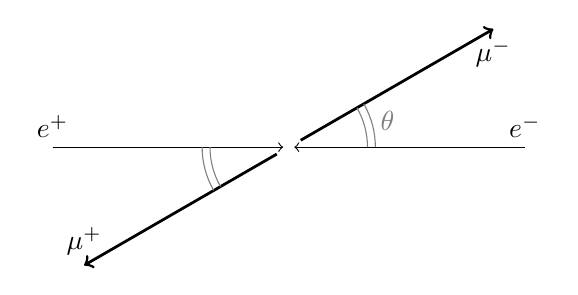
\begin{tikzpicture}
		\draw [shorten >= 2pt, ->] (180:3) node [above] {$e^+$} -- (0:0) coordinate (boom);
		\draw[shorten <= 2pt, <-] (boom) -- +(0:3) node [above] {$e^-$};

		\begin{scope}[shorten <= 5pt, ->, line width=1pt] 
			\draw (boom) -- +(30:3) node [below] {$\mu^-$};
			\draw (boom) -- +(210:3) node [above] {$\mu^+$};
		\end{scope}

		\begin{scope}[color=gray]
			\draw (1,0) arc (0:30:1);
			\draw (1.1,0) arc (0:30:1.1) node at (15:1.3) {$\theta$};

			\draw (-1,0) arc (180:210:1);
			\draw (-1.1,0) arc (180:210:1.1);

		\end{scope}

	\end{tikzpicture}
	\caption{Bhabha scattering}

\end{figure}

\begin{figure}
	\centering

	\subfloat[][As a function of $\cos\theta$.]{%
		\begin{tikzpicture}
\begin{axis}[%
	xlabel=$\cos\theta$,
	ylabel=$\sigma_\textup{tot}f(\cos\theta)$,
	smooth,
]
\addplot+ [mark=none,domain={-1:1}] {3*(1+x*x)/8};
\end{axis}
\end{tikzpicture}
	}

	\subfloat[][As a function of the angle.]{%
		\begin{tikzpicture}
\begin{axis}[%
	xlabel=$\theta$,
	x unit = degree,
	ylabel=$\sigma_\textup{tot}f(\theta)$,
	smooth
]
\addplot+ [mark=none,domain={0:180}] {3*(1+cos(x)*cos(x))/8};
\end{axis}
\end{tikzpicture}
	}
	\caption{Bhabha scattering cross section.}

\end{figure}



